\documentclass[aspectratio=169,12pt]{beamer}
\usepackage[utf8]{inputenc}
\usepackage{amsmath, amssymb}
\usepackage{booktabs}
\usepackage{colortbl}
\usepackage{hyperref}
\usepackage{makecell}
\usepackage{ragged2e}
\usepackage{bytefield}
\usepackage{tikz}
\usetikzlibrary{arrows.meta, positioning, shapes.geometric, calc, tikzmark, shapes.misc}
\usetheme{Madrid}

\title{Computer Structure}
\subtitle{System}
\author{Lihu Rappoport}
\date{}

% Clock macro - draws a clock at given location
\newcommand{\drawclock}[1]{
    \begin{scope}[shift={(#1)}]
        \draw[thick] (0,0) circle (0.12);
        \draw[thick] (0,0) -- (0,0.08);
        \draw[thick] (0,0) -- (0.05,-0.03);
    \end{scope}
}

\begin{document}

\frame{\titlepage}


\begin{frame}{Basic DRAM chip}
\textbf{DRAM:} 2D array of memory cells
\vspace{-0.2cm}

\begin{center}
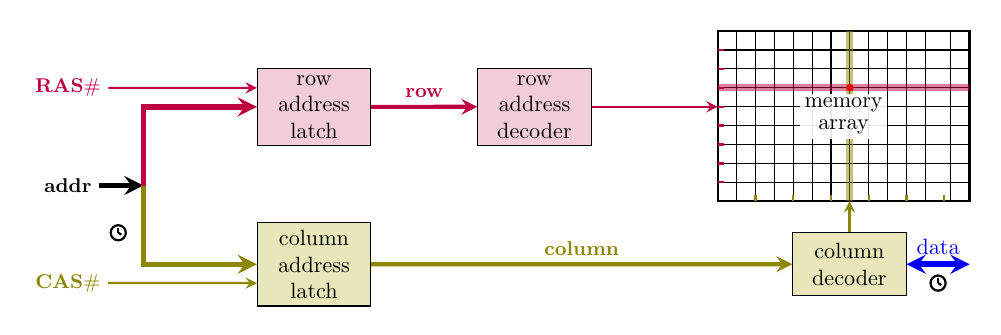
\begin{tikzpicture}[scale=0.8, transform shape,
    block/.style={draw, minimum width=1.8cm, minimum height=1cm, align=center},
    decoder/.style={draw, minimum width=1.8cm, minimum height=1.2cm, align=center},
    signal/.style={->, >=stealth, thick},
    label/.style={font=\small\bfseries}
]

% Origin point - move this to shift entire diagram
\coordinate (origin) at (0,25);

% Row Address Latch - positioned relative to origin
\node[block, text width=1.5cm, fill=purple!20] (rowlatch) at (origin) {row address latch};

% Column Address Latch - positioned relative to row latch
\node[block, text width=1.5cm, fill=olive!20] (collatch) at ([yshift=-2.5cm]rowlatch) {column address latch};

% Row Address decoder - positioned relative to row latch
\node[decoder, text width=1.5cm, fill=purple!20] (rowdecoder) at ([xshift=3.5cm]rowlatch) {row address decoder};

% Column decoder - positioned relative to column latch
\node[block, text width=1.5cm, fill=olive!20] (coldecoder) at ([xshift=8.5cm]collatch) {column decoder};

% Memory array - positioned relative to decoders
\coordinate (array_corner) at ([xshift=2cm, yshift=1.2cm]rowdecoder.east);
\draw[thick] (array_corner) rectangle ([xshift=4cm, yshift=-2.7cm]array_corner);
\foreach \x in {0.3,0.6,0.9,1.2,1.5,1.8,2.1,2.4,2.7,3,3.3,3.7} {
    \draw ([xshift=\x cm]array_corner) -- ([xshift=\x cm, yshift=-2.7cm]array_corner);
}
\foreach \y in {-0.3,-0.6,-0.9,-1.2,-1.5,-1.8,-2.1,-2.4} {
    \draw ([yshift=\y cm]array_corner) -- ([xshift=4cm, yshift=\y cm]array_corner);
}

% Input signals - positioned relative to latches
\node[label, purple] (ras) at ([xshift=-3cm, yshift=0.3cm]rowlatch.west) {RAS$\#$};
\draw[signal, purple] (ras) -- (ras -| rowlatch.west);

\node[label, olive] (cas) at ([xshift=-3cm, yshift=-0.3cm]collatch.west) {CAS$\#$};
\draw[signal, olive] (cas) -- (cas -| collatch.west);

% Address in the middle between the two latches
\node[label] (addr) at ($(rowlatch.west)!0.5!(collatch.west) + (-3,0)$) {addr};
\coordinate (addr_split) at ($(rowlatch.west)!0.5!(collatch.west) + (-1.8,0)$);

\draw[signal, line width=2pt] (addr.east) -- (addr_split);
% Branch to row and column latches
\draw[signal, purple, line width=2pt] (addr_split) -- (addr_split |- rowlatch.west) -- (rowlatch.west);
\draw[signal, olive, line width=2pt] (addr_split) -- (addr_split |- collatch.west) -- (collatch.west);

% Clock symbol relative to addr_split
\drawclock{$(addr_split) + (-0.4,-0.75)$}

% Connections between blocks
\draw[signal, purple, line width=1.5pt] (rowlatch.east) -- node[above, font=\small\bfseries, purple] {row} (rowdecoder.west);
\draw[signal, olive, line width=1.5pt] (collatch.east) -- node[above, font=\small\bfseries, olive] {column} (coldecoder.west);

% Row decoder to memory array with highlighted row
\draw[signal, purple] (rowdecoder.east) -- (rowdecoder.east -| array_corner);
% Draw wordlines and highlight one
\foreach \y in {-0.3,-0.6,-0.9,-1.2,-1.5,-1.8,-2.1,-2.4} {
    \draw[purple, thick] ([yshift=\y cm]array_corner) -- ++(0.1,0);
}
% Highlight one row
\draw[purple, line width=2.5pt, opacity=0.5] ([yshift=-0.9cm]array_corner) -- ([xshift=4cm, yshift=-0.9cm]array_corner);

% Column decoder to memory array with highlighted column
\coordinate (array_bottom) at ([yshift=-2.7cm]array_corner);
\draw[signal, olive] (coldecoder.north) -- (coldecoder.north |- array_bottom);
% Draw bitlines and highlight one
\foreach \x in {0.6,1.2,1.8,2.4,3,3.6} {
    \draw[olive, thick] ([xshift=\x cm, yshift=-2.7cm]array_corner) -- ++(0,0.1);
}
% Highlight one column
\draw[olive, line width=2.5pt, opacity=0.5] ([xshift=2.1cm]array_corner) -- ([xshift=2.1cm, yshift=-2.7cm]array_corner);

% Mark intersection
\fill[red] ([xshift=2.1cm, yshift=-0.9cm]array_corner) circle (0.06);

% Data I/O - horizontal arrow
\draw[signal, blue, line width=2pt, <->] 
  (coldecoder.east) 
    -- node[midway, above, blue]{data} 
  ++(1,0);

% Clock symbol near data - relative to coldecoder
\drawclock{$(coldecoder.east) + (0.5,-0.3)$}

\node[
  align=center, 
  fill=white, 
  fill opacity=0.9,   % background 50% transparent
  text opacity=1,     % text fully visible
  inner sep=2pt
] at ([xshift=2cm, yshift=-1.35cm]array_corner) {memory\\[-2]array};

\end{tikzpicture}
\end{center}

\vspace{-0.2cm}
\textbf{DRAM access sequence:}
\begin{enumerate}
\item Row address on bus → Assert RAS$\#$ to latch row
\item Column address on bus → Assert CAS$\#$ to latch column (after t$_{RCD}$ delay)
\item Data available after CAS latency (CL)
\end{enumerate}

\end{frame}
\end{document}